%*******************************************************************************
%****************************** Second Chapter *********************************
%*******************************************************************************
\graphicspath{{Chapter3/Figs/}}

\setcounter{chapter}{6}
\chapter*{Resultados y Discusión Capítulo 3} 
\addcontentsline{toc}{chapter}{Resultados y Discusión Capítulo 3}

{\LARGE Estudios de la evolución y biogénesis de miARNs}


\section{Introducción}


\section{Resultados y Discusión}

%~ ################################################# 
%~ Enfoque bioinformático para el estudio de la
%~ evolución y biogénesis de miARNs en plantas
%~ #################################################

\subsection{Enfoque bioinformático para el estudio de la evolución y biogénesis de miARNs en plantas}

Que los precursores de miARNs en plantas sean procesados de diferentes maneras \citep{Bologna2013}, nos llevó a especular que su patrón de evolución también puede ser diferente y podrían estar vinculados a su mecanismo de procesamiento.
Es por esto que elaboramos una estrategia bioinformática para caracterizar la relación entre la evolución de los precursores de miARNs en plantas y los mecanismos de procesamiento determinados previamente.

\subsubsection{Estrategia}

La metodología utilizada se detalla en la sección \ref{ref_evolution} y primero la utilizamos para estudiar precursores de miARNs conservados en dicotiledóneas. 
La misma consta de los siguientes pasos:

\begin{itemize}
    \item Búsqueda de ortólogos para cada miembro de cada familia de Arabidopsis de  precursores de miARNs conservados en plantas
    \item Extensión de las secuencias
    \item Alineamiento de secuencia primaria
    \item Alineamiento de secuencia teniendo en cuenta estructura secundaria
    \item Búsqueda de motivos conservados
    \item Representación gráfica de los precursores
\end{itemize}

\subsubsection{Búsqueda de ortólogos de precursores de miARNs}

Las secuencias de los precursores de miARNs en miRBASE rara vez son validadas experimentalmente, de hecho muchas de ellas son el resultado de predicciones computacionales de estructuras en forma de tallo y burbuja que incluye el miARN maduro, pero que no se extiende muchas bases más allá de el mismo \cite{Kozomara2014}.
Esto lleva a anotaciones erróneas de los precursores de miARNs.
Además para cada miembro de cada familia de \textit{A. thaliana} no es trivial asignarle un ortólogo en otra especie teniendo en cuenta la anotación de miRBASE.

Por esto, primero realizamos una búsqueda de ortólogos para cada miembro de cada familia de \textit{A. thaliana} y empezamos nuestro análisis con una definición arbitraria de los precursores de plantas incluyendo 150 nt fuera del par miARN/miARN*.
Para la búsqueda de ortólogos, extensión de la secuencia y el posterior análisis de los precursores, utilizamos datos genómicos de plantas extraídos de Phytozome. 

Para la mayoría de los miembros de cada familia de precursores pudimos detectar ortólogos en otras especies. 
Teniendo en cuenta las 30 dicotiledóneas utilizadas en este estudio, en promedio, se encontraron ortólogos para cerca de 20 especies para cada precursor de miARN de \textit{A. thaliana} (Figura \ref{fig:dicots_species}).

\begin{figure}[htbp!] 
    \centering    
    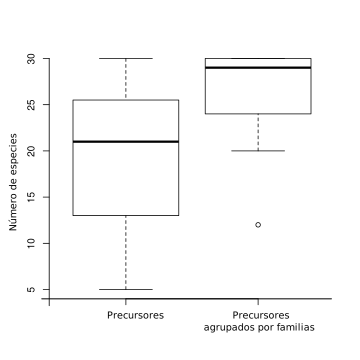
\includegraphics[width=.5\textwidth]{dicots_species.png}
    \caption[Especies detectadas]{Cantidad de especies detectadas.
    Esta figura muestra la distribución de la cantidad de especies donde se encuentran ortólogos de precursores de miARNs.
    A la izquierda se muestra la distribución de especies por miembro de familias de precursores de miARNs donde se detecta el ortólogo de \textit{A. thaliana}.
    A la derecha se agruparon todos los miembros de una misma familia y se muestra la distribución de la cantidad de especies donde se detecta un ortólogo de \textit{A. thaliana}}
    \label{fig:dicots_species}
\end{figure}

Algunos familias de miARNs se han diversificado durante la evolución, donde en algunas especies un miARN puede encontrarse como un único gen y en otras especie el mismo miARN puede encontrarse en múltiples miembros.
Por ejemplo, el miR396 en Arabidopsis está constituido por dos miembros, miR396a y miR396b mientras que en en el caso de arroz existen 8 miembros, nombrados del miR396a al miR396h.
Por esto, agrupamos a los miembros por familias y vimos la distribución de la cantidad de especies donde se detecta un ortólogo de los precursores de miARNs pertenecientes a \textit{A. thaliana} y en este caso vimos un alto número de especies detectadas para la mayoría de las familias de miARNs (Figura \ref{fig:dicots_species}).

\subsubsection{Alineamiento de los precursores en base a su secuencia primaria}

Comenzamos con los alineamientos múltiple de cada miembro de las familias de precursores de miARNs conservadas en dicotiledóneas.
Primero, realizamos el alineamiento en base a su secuencia primaria utilizando la herramienta T-Coffee \citep{pmid10964570}.
En la Figura \ref{fig:miR172a_tcoffee} se muestra el alineamiento del precursor del miR172a en distintas especies coloreado en base a la conservación evolutiva de la secuencia primaria.
Se puede observar que el miR172a maduro y el miR172a* están muy conservados en las distintas especies, pero además se puede ver una cola de conservación que podría corresponder al tallo inferior del precusor (Figura \ref{fig:miR172a_tcoffee}).

\begin{landscape}
    \begin{figure}[htbp!] 
        \centering    
        \includegraphics[width=1.4\textwidth]{miR172a_tcoffee.png}
        \caption[Alineamiento del precursor del miR172a.]{Alineamiento del precursor del miR172a. 
        Se muestra el alineamiento del precursor del miR172a en distintas especies. 
        En colores se muestra la conservación de la secuencia primaria, donde azul más oscuro denota mayor conservación y naranja menor conservación.
        Se muestran $\sim$60 bases por debajo del dúplex miARN/miARN* y los alineamientos están separados en dos líneas para una mejor representación.}
         \label{fig:miR172a_tcoffee}
    \end{figure}
\end{landscape}

Para poder corroborar esto y obtener información adicional sobre la conservación de los precursores, realizamos la predicción de estructura secundaria utilizando la herramienta RNAfold \citep{pmid22115189} (Figura \ref{fig:miR172a_rnafold}).
Además realizamos nuevamente los alineamientos pero considerando la estructura secundaria de los precursores, utilizando la herramienta R-Coffee \citep{pmid18292307}.

En la Figura \ref{fig:miR172a_rnafold} se puede observar que existe un patrón que comparten los precursores en la región debajo del miARN/miARN*.
No es simple reconocer patrones similares mirando los precursores de esta manera.
Además la cantidad de precursores estudiados en esta parte del trabajo de Tesis dificulta aún más este tipo de análisis.

\begin{landscape}
    \begin{figure}[htbp!] 
        \centering    
        \includegraphics[width=1.4\textwidth]{miR172a_rnafold.png}
        \caption[Estructura secundaria del miR172a en distintas especies]{
        Estructura secundaria del miR172a en distintas especies.
        Se muestra la estructura secundaria de los precursores del miR172a en distintas especies, calculados con la herramienta RNAfold.
        }
        \label{fig:miR172a_rnafold}
    \end{figure}
\end{landscape}

Para poder reconocer fácilmente la región conservada dentro del precursor y poder analizar más en detalle estos patrones de conservación, decidimos agrupar toda esta información
 generada a partir de los alineamientos de secuencia primaria y estructura secundaria en un gráfico circular como se muestra en la figura \ref{fig:miR172a_circos}.
Estos gráficos se hicieron utilizando el paquete Circos \citep{pmid19541911}.
 
En dicha figura se muestra el Circos del miR172a a modo de ejemplo.
Para representar el precursor, se tomaron 60 nt por debajo del dúplex miARN/miARN*.
En el anillo exterior se representa en colores el grado de conservación de la secuencia consenso a partir de los alineamientos en base a su secuencia primaria.
Además se muestran las bases del precursor de \textit {A. thaliana}.
Luego en el anillo interior se representa, mediante un histograma, la frecuencia de bases apareadas y desapareadas para cada posición del precursor en las distintas especies.
Con líneas de distinto espesor se muestra la interacción de las bases del precursor considerando la estructura secundaria. 
Fuera del anillo exterior se marca la secuencia del miARN y miARN*.

Realizamos los Circos para visualizar de manera simple los precursores de miARNs en distintas especies de plantas.
Y los utilizamos para caracterizar la relación entre los patrones de conservación y los mecanismos de procesamiento determinados previamente.


\begin{figure}[htbp!] 
    \centering    
    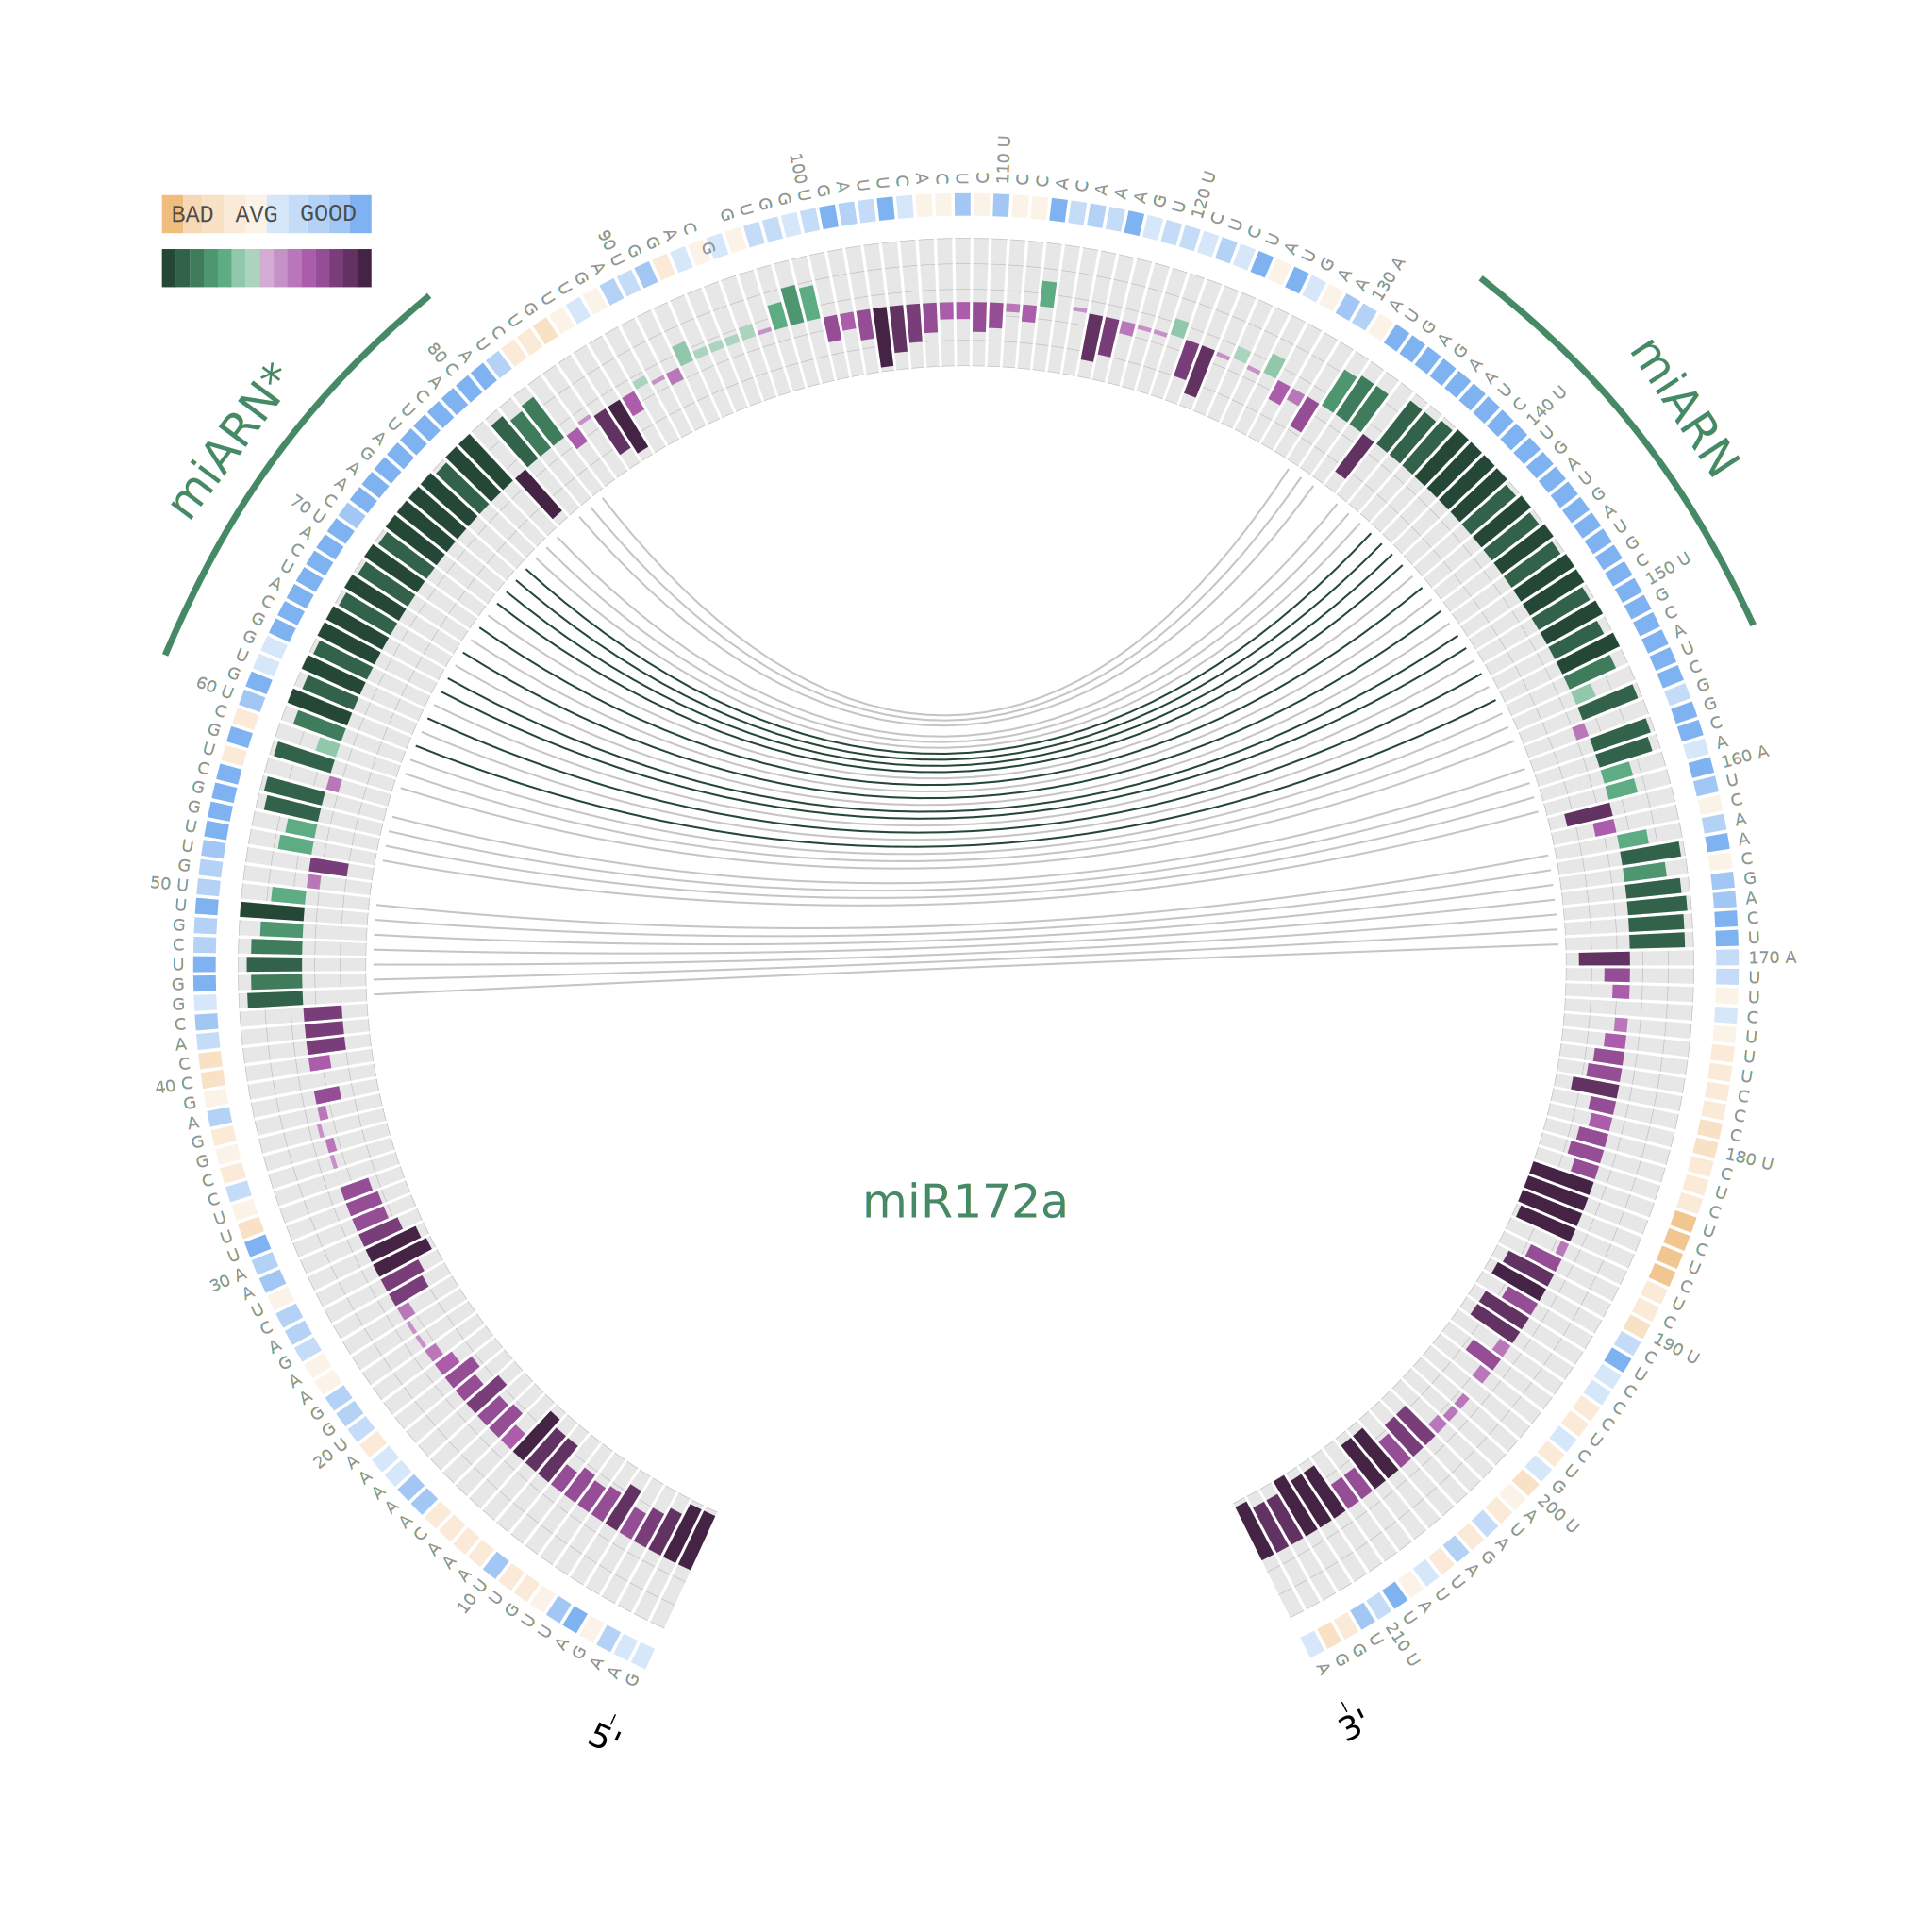
\includegraphics[width=1\textwidth]{miR172a_circos.png}
    \caption[Circos del miR172a]{Circos del miR172a.
En el anillo exterior se representa en colores el grado de conservación de la secuencia consenso a partir de los alineamientos en base a su secuencia primaria.
Además se muestran las bases del precursor de \textit {A. thaliana}.
Luego en el anillo interior se representa, mediante un histograma, la frecuencia de bases apareadas y desapareadas para cada posición del precursor en las distintas especies.
Con líneas de distinto espesor se muestra la interacción de las bases del precursor considerando la estructura secundaria. 
Fuera del anillo exterior se marca la secuencia del miARN y miARN*.
   }
     \label{fig:miR172a_circos}
\end{figure}

Por último, para cada precursor en distintas especies, realizamos una búsqueda de motivos conservados con la herramienta MEME \citep{pmid22115189} (Figura \ref{fig:miR172_meme}).
Hicimos esto para poder ver de manera visual cuáles eran los patrones comunes entre las distintas especies y donde se localizaban dentro del precursor.
Esta búsqueda de motivos la hicimos de diferentes maneras, la primera permitiendo encontrar hasta 2 motivos conservados en los precursores de distintas especies.


\begin{landscape}
    \begin{figure}[htbp!] 
        \centering    
        \includegraphics[width=1.4\textwidth]{miR172_meme.png}
        \caption[MEME del miR172a]{
			\textbf{MEME del miR172a.}
        Se muestra el MEME donde se pueden observar los motivos conservados dentro de los precursores del miR172a en distintas especies.
        En color rojo el primer motivo conservado comprende parte del miR172 (logo 1).
        El segundo motivo más conservado comprende parte del miR172* (logo 2).
        }
        \label{fig:miR172_meme}
    \end{figure}
\end{landscape}

\subsubsection{Mecanismo de base a loop cortos}

En los precursores con un mecanismo corto de base a loop, un loop interno seguido por un tallo inferior de $\sim$15nt especifica la posición del primer corte.
A pesar de que el tallo puede contener bulges, la transición de un loop interno (simple hebra) al tallo inferior es bastante marcada, y tres pares de bases apareadas generalmente definen el comienzo del tallo inferior del precursor \citep{Mateos2010,Bologna2013}.
El segundo corte procede a una distancia fija de $\sim$21 nt desde la posición del primer corte.

Para la mayoría de los precursores procesados con este mecanismo pudimos observar el mismo patrón de conservación de estructura primaria y similares patrones de estructura secundaria.
Para los precursores del miR172a (Figura \ref{fig:miR172a_circos} y el miR390a \ref{fig:miR390a_circos}), mediante la estrategia pudimos encontrar precursores en las 30 especies utilizadas.
En ambos casos, se pudo observar que la región con mayor conservación conincide con el duplex miARN/miARN* pero además se puede ver una región conservada por debajo del dúplex, que coincide con el tallo inferior.

Otra ventaja de esta forma de representar a los precursores con la conservación entre especies, es que visualmente se puede reconocer facilmente las posiciones donde existen "mismatches" conservados. 
Por ejemplo en el Circos del miR172, se puede observar un mismatch en la primer posición del miARN con la posición 19 del miARN*.
Esta interacción es A-A y se mantiene sin variaciones en todas las especies (Figura \ref{fig:miR172a_circos}).
Esto podría ser interesante estudiarlo en detalle donde se podría generar un precursor mutante donde esas bases en particular estén apareadas y luego ver si esto afecto o no el procesamiento del precursor.  
Además notamos que este patrón de conservación se puede observar independientemente si el miARN maduro está en la hebra 5' (Figura \ref{fig:miR172a_circos}) o si está en la hebra 3' (Figura \ref{fig:miR390a_circos}).

A diferencia de los precursores que tienen un mecanismo de loop a base, donde el tallo superior es fundamental para el su procesamiento, los precursores que se procesan cortos de base a loop no tienen el tallo superior conservado.
Y mediante la búsqueda de motivos conservados, pudimos observar que el tamaño del tallo superior y del loop es muy variado en un mismo precursor en distintas especies, donde los mismos puede ir desde los 40nt hasta 115nt (Figura \ref{fig:miR172_meme}).


\begin{figure}[htbp!] 
    \centering    
    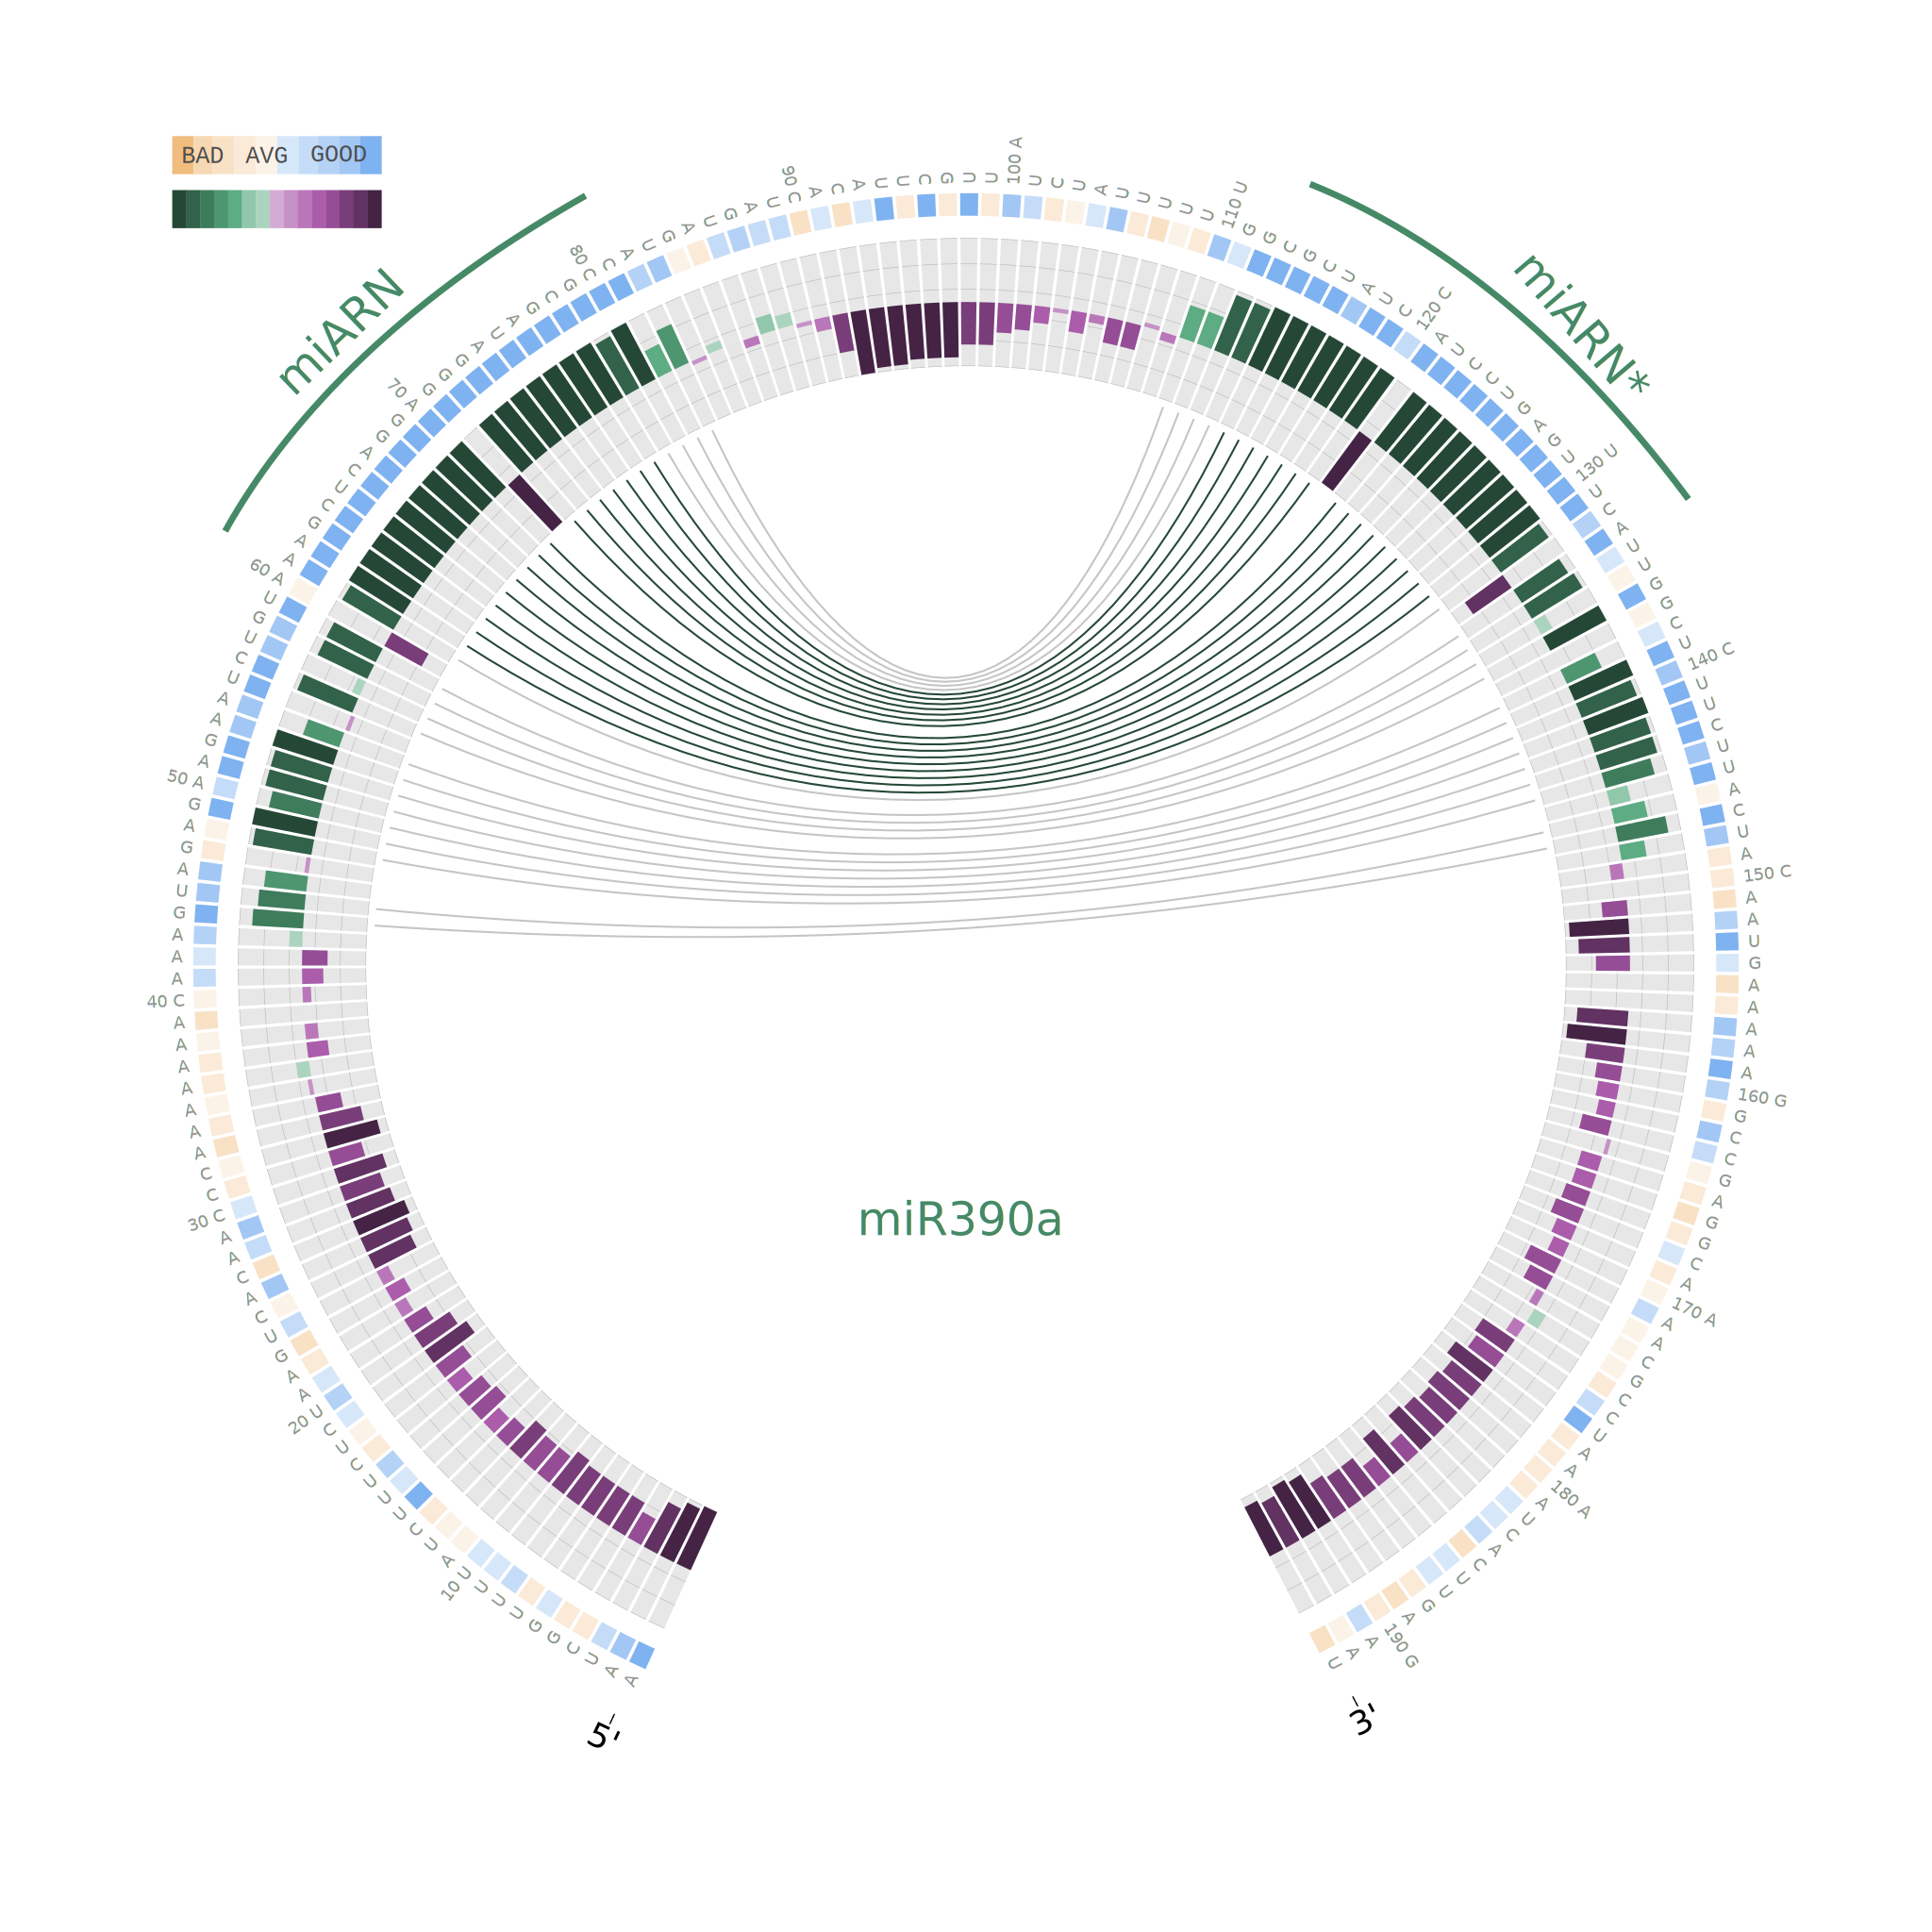
\includegraphics[width=1\textwidth]{miR390a_circos.png}
    \caption[Circos del miR172a]{Circos del miR390a.}
     \label{fig:miR390a_circos}
\end{figure}

\subsubsection{Mecanismo de base a loop secuenciales}

En estos precursores, con un mecanismo secuencial de base a loop, el primer corte procede como en los cortos de base a loop, pero luego son necesario dos cortes más para liberar el miARN, generando en el proceso niveles bajos de RNA pequeños adicionales \citep{Bologna2013}.
Este es el caso de algunos miembros de la  familias del miR169, que tiene en total 14 miembros siendo la familia más grande de \textit{A. thaliana}.
Un estudio en detalle de los precursores del miR169b/d/e/f/g mostró que los sitios de cortes del precursor estaban localizados 21 nt por debajo del lado proximal del dúplex miARN/miARN*.
Esta es la distancia esperada entre dos cortes de DCL1, sugeriendo que estos precursores eran procesados por más de dos cortes de la encima \citep{Bologna2013}.

La familia del miR394 también es procesada de la misma manera y comparten similares patrones de estructura secundaria, donde se ve el tallo inferior largo bien estructurado (Figura \ref{fig:seqBTL_circos}).
Si observamos el patrón de conservación de secuencia primaria podemos ver que la región del dúplex miARN/miARN está muy conservada, pero además podemos observar que debajo del dúplex existe otra región conservada que coincide con el tallo inferior largo que presentan estos precursores (Figura \ref{fig:seqBTL_circos}).

%~ 394b 26 especies
%~ 319b 22 especies

\begin{landscape}
	\begin{figure}
	\centering
	\begin{subfigure}{.75\textwidth}
	  \centering
	  \includegraphics[width=.9\linewidth]{miR169b_circos.png}
	  \caption{Precursor del miR169b}
	  \label{subfig:miR169b_circos}
	\end{subfigure}%
	\begin{subfigure}{.75\textwidth}
	  \centering
	  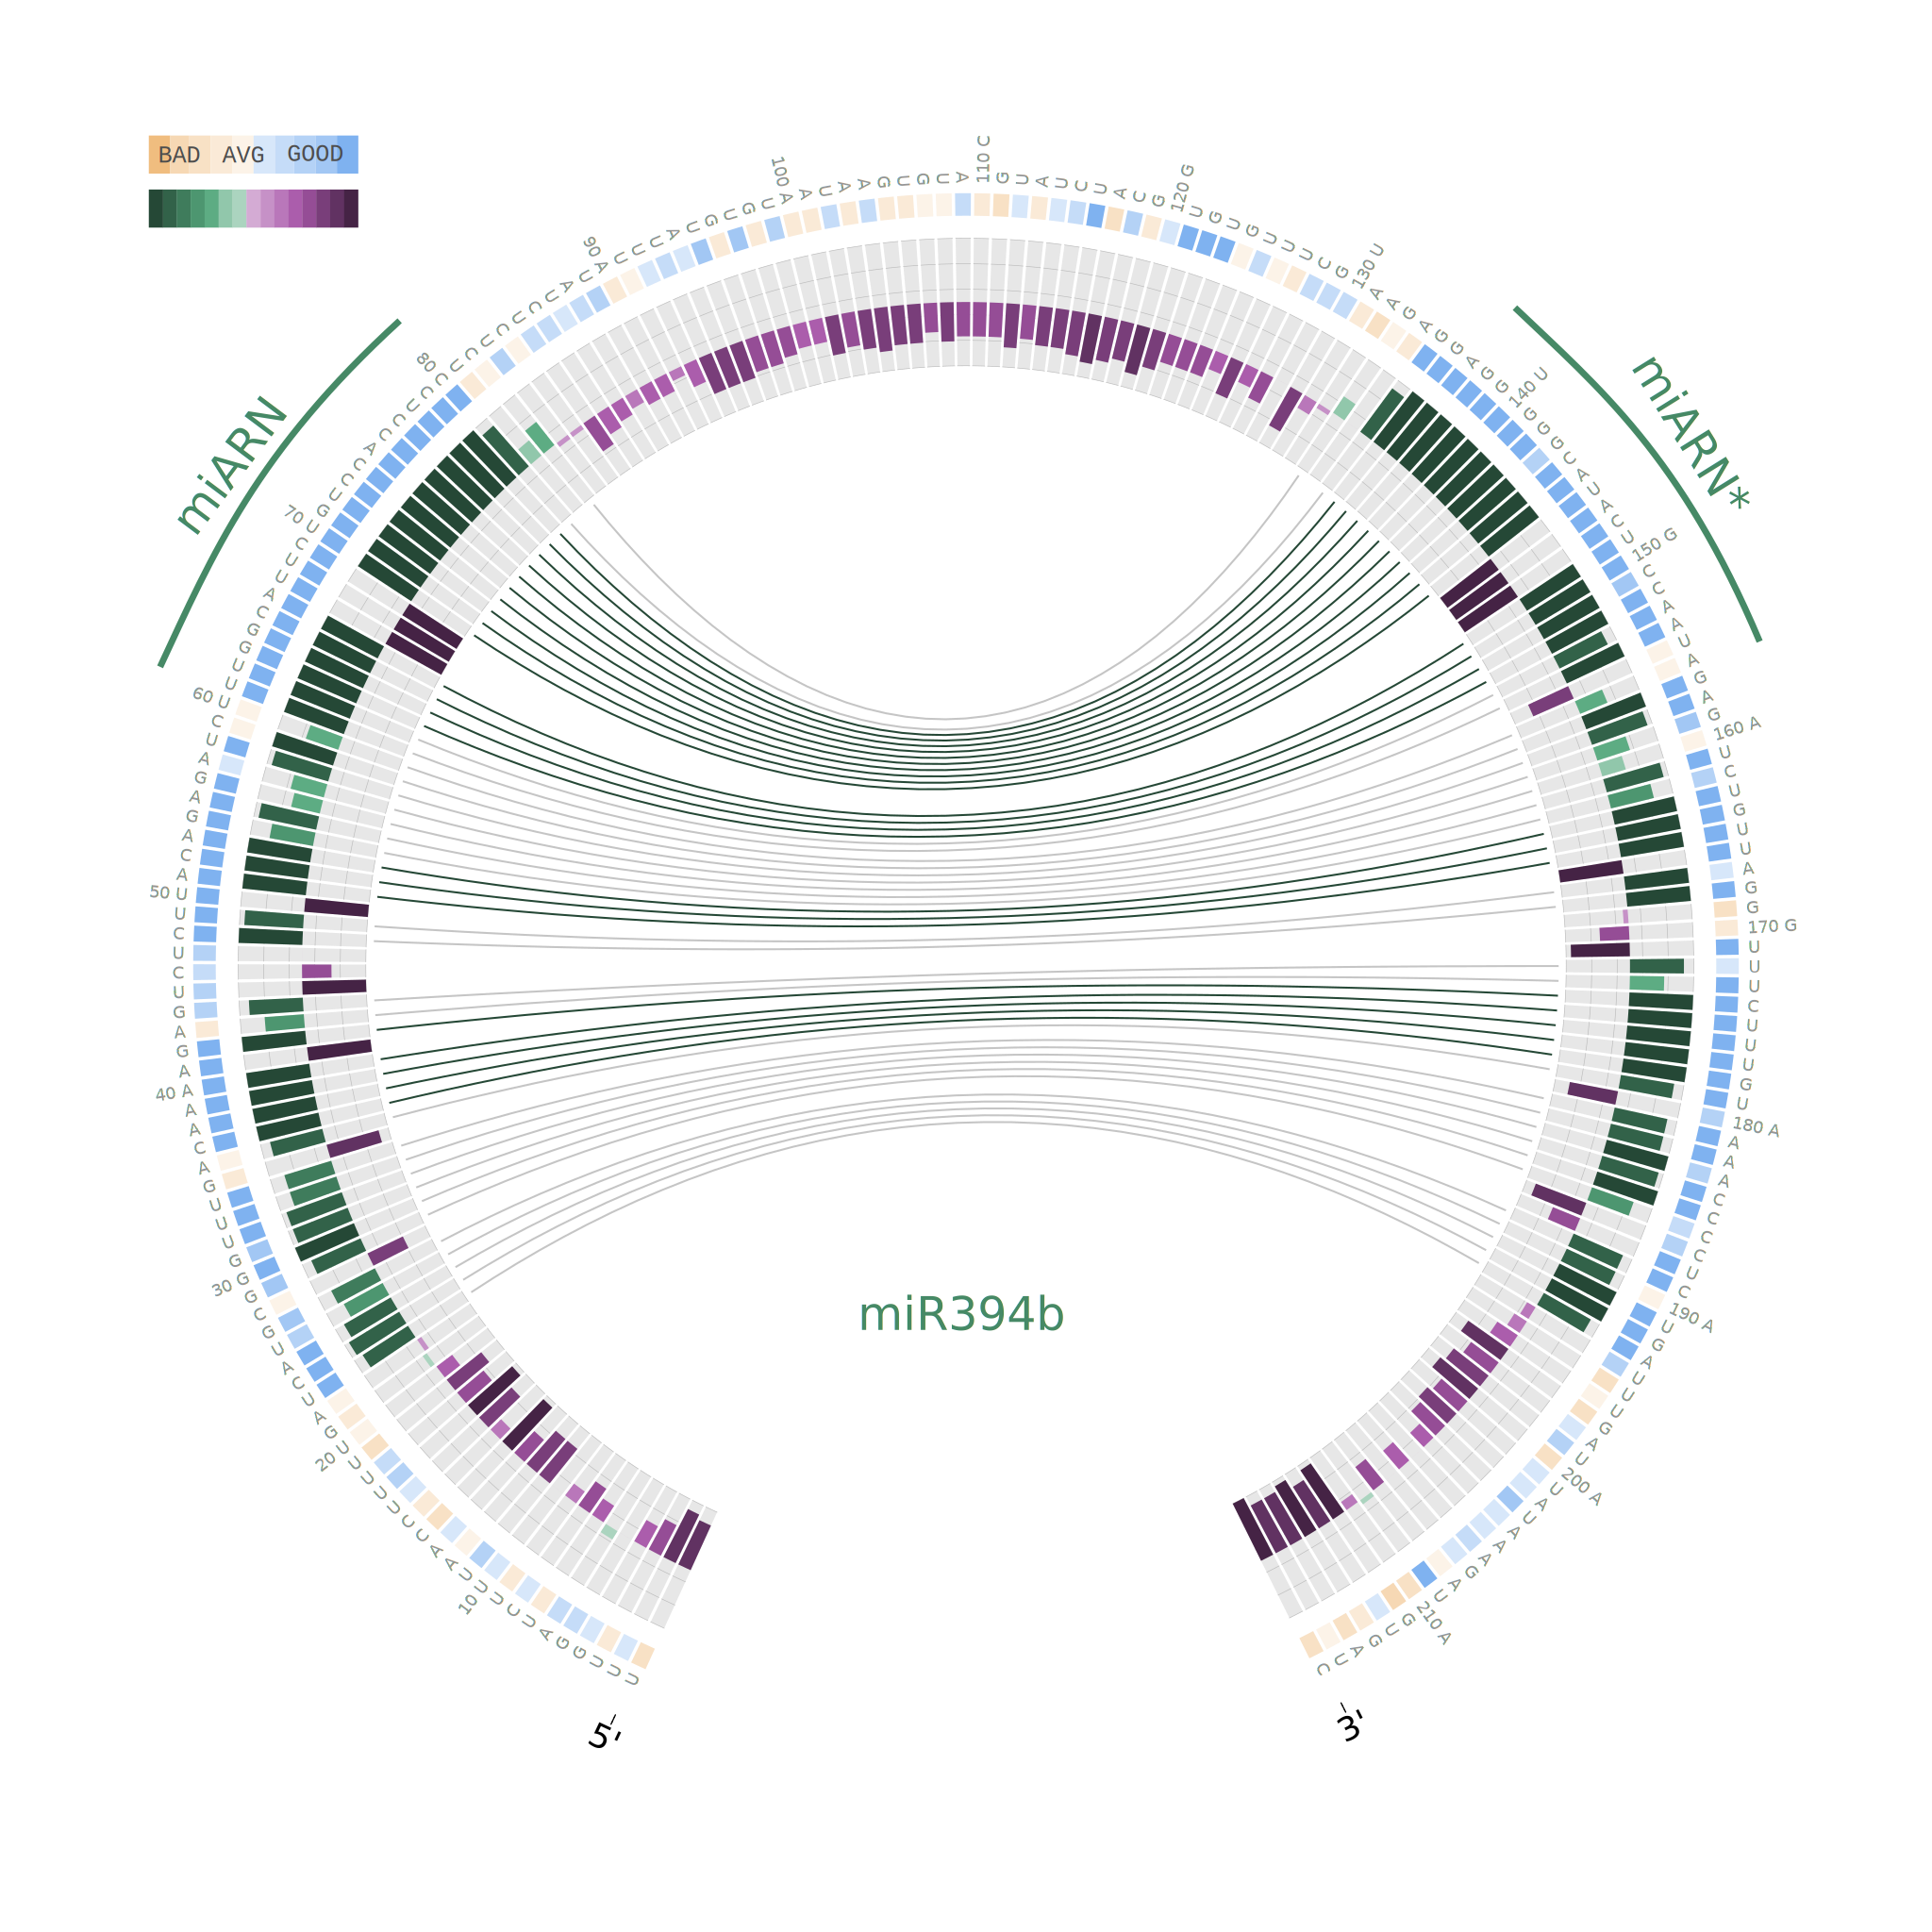
\includegraphics[width=.9\linewidth]{miR394b_circos.png}
	  \caption{Precursor del miR394b}
	  \label{subfig:miR394b_circos}
	\end{subfigure}
	\caption{Circos de precursores con mecanismos de procesamientos secuenciales de base a loop}
	\label{fig:seqBTL_circos}
	\end{figure}
\end{landscape}


\subsubsection{Mecanismo de loop a base cortos}

En los precursores con un mecanismo \textbf{cortos de loop a base}, el procesamiento es guiado por un tallo superior, y son necesarios dos cortes para liberar el miARN maduro.
La región terminal de estos precursores tienen una largo conservado de $\sim$42, donde incluye un loop pequeño \citep{Bologna2013} a diferencia de los precursores procesados dee base a loop, donde esta región es variable en tamaño.

En este caso mostramos los Circos para el precursor del miR157a, que fue encontrado en 30 especies, y para el precursor del miR160a también encontrado en 30 especies. 
En los precursores que se procesan cortos de base a loop observamos que presentan una región conservada que corresponde al tallo superior además de la región que comprende al dúplex miARN/miARN* (Figura \ref{fig:seqBTL_circos}).
A diferencia de los precursores que se procesan de la base al loop, estos precursores no presentan el tallo inferior ni estructurado ni conservado y esto se puede observar en ambos casos; en el miR157a (Figura \ref{subfig:miR157a_circos}) y del miR160a (Figura \ref{subfig:miR160a_circos}).


\begin{landscape}
	\begin{figure}
	\centering
	\begin{subfigure}{.75\textwidth}
	  \centering
	  \includegraphics[width=.9\linewidth]{miR157a_circos.png}
	  \caption{Precursor del miR157a}
	  \label{subfig:miR157a_circos}
	\end{subfigure}%
	\begin{subfigure}{.75\textwidth}
	  \centering
	  \includegraphics[width=.9\linewidth]{miR160a_circos.png}
	  \caption{Precursor del miR160a}
	  \label{subfig:miR160a_circos}
	\end{subfigure}
	\caption{Circos de precursores con mecanismos de procesamientos cortos de loop a base}
	\label{fig:srLTB_circos}
	\end{figure}
\end{landscape}

\subsubsection{Mecanismo de loop a base secuenciales}

En los precursores con un mecanismo \textbf{secuencial de loop a base}, cuatro cortes secuenciales por DCL1 son los encargados de procesar los precursores de miARNs.
En general, estos precursores muestran un tallo largo superior, del cual otros ARNs pequeños son generados \citep{pmid19850910,Bologna2009,Bologna2013}.

En este caso estudiamos la familia del miR319 y del miR159 y en particular mostramos al miR319a (Figura \ref{subfig:miR319a_circos}) y al miR159b (Figura \ref{subfig:miR159b_circos}).
Pudimos reconocer el tallo superior conservado y estructurado.
Además se pudo observar que los ARNs pequeños, que se originan del procesamiento de estos precursores, están conservados de la misma manera que el miARN y el miARN* (Figura \ref{fig:seqLTBL_circos}).

\begin{landscape}
	\begin{figure}
	\centering
	\begin{subfigure}{.75\textwidth}
	  \centering
	  \includegraphics[width=.9\linewidth]{miR319a_circos.png}
	  \caption{Precursor del miR319a}
	  \label{subfig:miR319a_circos}
	\end{subfigure}%
	\begin{subfigure}{.75\textwidth}
	  \centering
	  \includegraphics[width=.9\linewidth]{miR159b_circos.png}
	  \caption{Precursor del miR159b}
	  \label{subfig:miR159b_circos}
	\end{subfigure}
	\caption{Circos de precursores con mecanismos de procesamientos secuenciales de loop a base}
	\label{fig:seqLTBL_circos}
	\end{figure}
\end{landscape}


\subsubsection{Procesamiento mixto de miembros de la familia del miR170/miR171}

En general, se sabe que diferentes miembros de una misma familia de miARNs comparten la misma vía de biogenésis. 
Esta observación no sorprende ya que se cree que las familias de miARNs se expanden por eventos de duplicación de un gen ancestral \citep{pmid15565108}.
Sin embargo, ciertos el procesamiento de miembros de ciertas familias pueden variar de uno a otro \citep{Bologna2013}.
Esto sucede, por ejemplo,en la familia del miR171 donde en \textit{A. thaliana} existen 4 miembros. 
El precursor del miR171a es procesado de base a loop, mientras que los precursores del miR171b y miR171c son procesados de loop a base.

Nos pusimos a analizar esta familia en detalle para ver si los patrones de conservación y estructura secundaria eran diferentes o no.
Observamos que el miR171a, que es procesado corto de base a loop, tiene un patrón de conservación similar a los precursores procesados de base a loop, donde el tallo inferior es estructurado y conservado (Figura \ref{subfig:miR171a_circos}).
Por el contrario el miR171c, que es procesado corto de loop a base, muestra conservación en el tallo superior, que además es estructurado, y no así el tallo inferior (Figura \ref{subfig:miR171c_circos}).


%~ #######
%~ ##### TENGO QUE REHACER EL MIR171A en el lab
%~ #######

\begin{landscape}
	\begin{figure}
	\centering
	\begin{subfigure}{.65\textwidth}
	  \centering
	  \includegraphics[width=.9\linewidth]{miR171c_circos.png}
	  \caption{Precursor del miR171c. Procesamiento de loop a base. }
	  \label{subfig:miR171c_circos}
	\end{subfigure}
	\begin{subfigure}{.65\textwidth}
	  \centering
	  \includegraphics[width=.9\linewidth]{miR171a_circos.png}
	  \caption{Precursor del miR171a. Procesamiento de base a loop.}
	  \label{subfig:miR171a_circos}
	\end{subfigure}
	\caption{Procesamiento mixto de miembros de la familia del miR170/miR171}
	\label{fig:familia_miR171_circos}
	\end{figure}
\end{landscape}


\subsubsection{Mutaciones puntuales afectan el procesamiento de miARNs en plantas}
%~ Natural Variation in Biogenesis
%~ Efficiency of Individual
%~ Arabidopsis thaliana MicroRNAs

Se ha demostrado recientemente que un polimorfismo de origen natural que ocurre en el gen del miR164a afecta a la forma de la hoja y la arquitectura del vástago en \textit{A. thaliana}, con los efectos de ser modificados por loci adicionales en el genoma \citep{pmid22206705}.
Una sustitución única en un par de bases en la secuencia complementaria del miARN altera la estabilidad predicha del dúplex miARN/miARN*.
Se reduce con ello, en gran medida, la acumulación del miARN maduro, probablemente porque interfiere en el procesamiento del precursor.
Además se demostró en ese mismo artículo que no es una rara excepción y que las cepas naturales de \textit{A. thaliana} albergan decenas de polimorfismos similares que afectan al procesaciemiento de una amplia gama de precusores de miARNs.

Es por esto que nos pusimos a estudiar en detalles al precursor del miR164a.
A nivel de secuencia los alelos de Col-0 y C24 son diferentes sólo por un par de polimorfismos simples.
Uno de ellos afecta a una C en el miARN* que aparea con una G en la posición dos del miARN (nos referimos a esta posición como *2) (Figura \ref{fig:miR164_base_pairing}).

\begin{figure}[htbp!] 
	\centering    
	\includegraphics[width=0.6\textwidth]{miR164_base_pairing.png}
	\caption[Apareamiento de bases en el precursor del miR164a]{
		\textbf{Apareamiento de bases en el precursor del miR164a.}
		El miARN se muestra en rojo y el miARN* en azul.
		En la posición *2, el alelo alternativo C24 se muestra en naranja.
	}
	\label{fig:miR164_base_pairing}
\end{figure}

Se puede ver que el remplazo de una G:C en el miR164$a^{Col-0}$ por un par no canónico G:U en el miR164$a^{C24}$, incrementa ligeramente la energía libre del plegado del precursor que cambia de -41.58 kcal/mol a -39.28 kcal/mol, pero no se modifica la estructura secundaria del miR164a (Figura \ref{fig:miR164_ss}). 

\begin{figure}[htbp!] 
	\centering    
	\includegraphics[width=0.3\textwidth]{miR164_ss.png}
	\caption[Estructura secundaria predicha del precursor del miR164a]{
	\textbf{Estructura secundaria predicha del precursor del miR164a.}
	La barra gris horizontal indica el polimorfismo, un G:C en Col-0 y un G:U en C24.
	Los colores indican probabilidad de pares de bases.
	}
	\label{fig:miR164_ss}
\end{figure}

Realizamos el Circos del miR164a en distintas especies para ver como era la conservación de la base en la posición 2* que hace que el precursor no pueda ser procesado de manera correcta.
Lo que pudimos observar es que dicha posición del miR164a* está conservada en dicotiledóneas y se mantiene sin cambios en todas las especies (Figura \ref{miR164a_circos}).
Además esa base está siempre apareada con la base correspondiente del miARN maduro, formando un G:C (Figura \ref{miR164a_circos} a la derecha)..

También se puede observar que en la secuencia del miR164a* existen mutaciones en distintas bases en distintas especies, pero no en la base que estamos estudiando.
Esto sugiere que esa base en particular es importante para la estabilidad del precursor y su buen procesamiento.

%~ \begin{landscape}
    \begin{figure}[htbp!] 
        \centering    
        \includegraphics[width=1\textwidth]{miR164a_circos.png}
        \caption[Circos del miR164a]{
			\textbf{Circos del miR164a}.
			A la izquierda se representa el Circos del miR164a.
			A la derecha el alineamiento del miR164a en distintas especies. 
			Con una flecha verde se destaca la posición *2 a estudiar, en el Circos y en el alineamiento.
        }
        \label{fig:miR164a_circos}
    \end{figure}
%~ \end{landscape}

En otro trabajó, se estudió un alelo mutante llamado miR394b-1, que tiene un mismatch en el stem inferior del precursor del miR394b \citep{pmid23333352}.
La mutante incrementa dramáticamente la terminación del meristema apical.   
En la figura \ref{fig:miR164_base_pairing} se muestra el apareamiento de bases en el precursor del miR394b y miR394b-1, donde el miARN se muestra en rojo y el miARN* en azul.
Y en naranja se muestra la posición de la mutación del precursor del miR394b-1 donde la G es reemplazada por una A con respecto al miR394b.
En este caso se mostró que los niveles de maduro en el precursor del miR394b-1 se ven fuertemente disminuídos aunque no completamente ausentes \citep{pmid23333352}. 

\begin{figure}[htbp!] 
	\centering    
	\includegraphics[width=0.6\textwidth]{miR394b_base_pairing.png}
	\caption[Apareamiento de bases en el precursor del miR394b]{
		\textbf{Apareamiento de bases en el precursor del miR394b.}
		El miARN se muestra en rojo y el miARN* en azul.
		En naranja se muestra la posición de la mutación G por A en el stem inferior del precursor del miR394b-1.
	}
	\label{fig:miR164_base_pairing}
\end{figure}

Para varios precursores de plantas hemos visto anteriormente que esa región que corresponde al stem inferior es crucial para su procesamiento.
En este caso mostramos el Circos correspondiente al miR394b, para poder visualizar que es lo que sucede con esta mutación puntual fuera del dúplex miARN/miARN* (Figura \ref{fig:miR394b_circos_aliniamientos}).
Vemos, como en el caso del miR164a, está mutación que afecta al procesamiento del precursor y a la acumulación del miARN maduro, está conservada en todas las especies estudiadas.
Esto sugiere que esta base es importante para el procesamiento y que no sólo mutaciones de una base dentro del dúplex miARN/miARN* pueden afectar el procesamiento, sino que mutaciones simples en el precursor puede afectar el reconocimiento de DCL1. 

%~ \begin{landscape}
\begin{figure}[htbp!] 
	\centering    
	\includegraphics[width=1\textwidth]{miR394b_circos_aliniamientos.png}
	\caption[Circos del miR394b]{
		\textbf{Circos del miR394b}.
		A la izquierda se representa el Circos del miR394b.
		A la derecha el alineamiento del miR394b en distintas especies. 
		Con una flecha verde se destaca la posición a estudiar, en el Circos y en el alineamiento.
	}
	\label{fig:miR394b_circos_aliniamientos}
\end{figure}
%~ \end{landscape}

%~ Por otro lado, se seleccionaron todos los precursores que codifican para miARNs de la misma familia y luego los analizamos en conjunto.

%~ \subsubsection{Procesamiento central?????}
%~ miR166b 
%~ \subsubsection{Compensatory mutation}
%~ miR164a
%~ miR394b

\subsubsection{Precursores en plantas monocotiledóneas}


\subsubsection{Precursores de animales}

Para esta parte del trabajo de Tesis, utilizamos genomas de distintos especies de \textit{Metazoa} entre ellos humanos, monos, rana, vaca y pez (Tabla \ref{table:db_metazoa}).
Y estudiamos que sucede con los precursores de miARNs conservados en animales.
Para esto partimos de los precursores de humanos definidos en miRBASE.

\begin{table}[!htbp]
\centering
\small
\caption{Especies de \textit{Metazoa} utilizadas}
\label{table:db_metazoa}
\begin{tabular}{c}
\rowcolor[HTML]{ECF4FF} 
\textbf{Animales}        \\
	Bos taurus               \\
	Canis familiaris         \\
	Equus caballus           \\
	Gallus gallus            \\
	Gorilla gorilla          \\
	Homo sapiens             \\
	Macaca mulatta           \\
	Monodelphis domestica    \\
	Mus musculus             \\
	Ornithorhynchus anatinus \\
	Petromyzon marinus       \\
	Sus scrofa               \\
	Xenopus tropicalis      
\end{tabular}
\end{table}
